\documentclass[dutch]{beamer}
\usepackage{babel}
\usepackage{graphicx}
\usepackage{epsfig}
\usepackage{color}
\usepackage{algorithmic}
\usepackage{multicol}

\usetheme{Rochester}
\useinnertheme{rounded}
\usefonttheme{structurebold}
\usecolortheme{beetle}

\newtheorem{stelling}[theorem]{Stelling}

\theoremstyle{definition}
\newtheorem{definitie}[theorem]{Definitie}

\theoremstyle{remark}
\newtheorem{opmerking}[theorem]{Opmerking}

\theoremstyle{example}
\newtheorem{voorbeeld}[theorem]{Voorbeeld}


\AtBeginSection[]{\plainframe{\tableofcontents[currentsection,hidesubsections]}}

\title{Similariteitsgebaseerd rangschikken van beelden in zoekmachines}
\author{Klaas Bosteels}
\date{Academiejaar 2005-2006}

\titlegraphic{\includegraphics[scale=1]{ugent.eps}}

\begin{document}

\plainframe{\titlepage}

\section{Inleiding}
\frame
{
  \frametitle{Situering}
  
  \begin{center}
  \includegraphics[width=\textwidth]{images/situering.eps}
  \end{center}
}
\frame
{
  \frametitle{Tekstgebaseerd zoeken van beelden}

  \begin{center}
  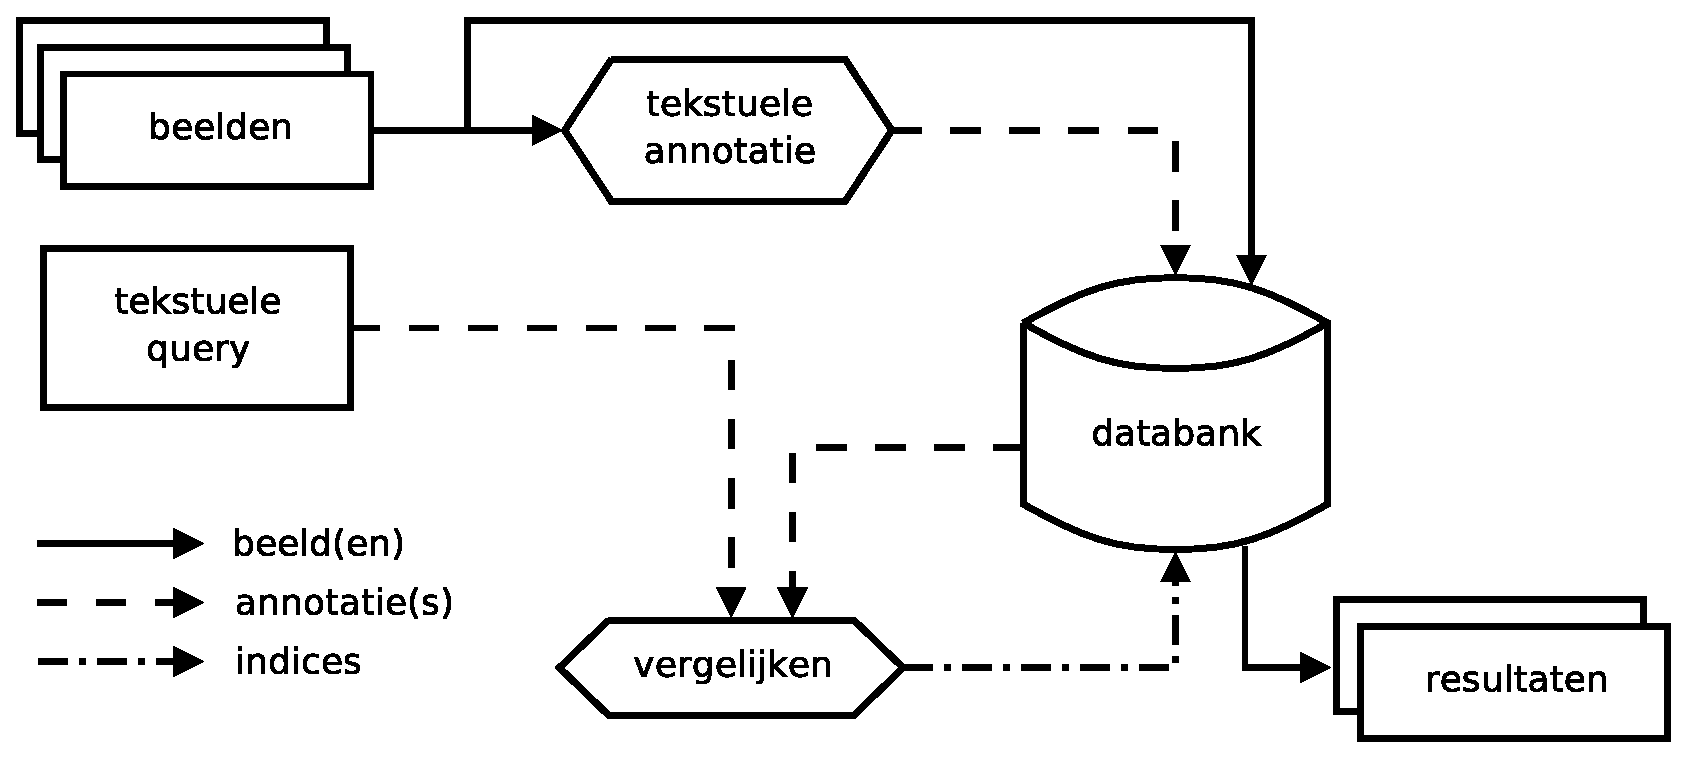
\includegraphics[width=\textwidth]{images/tbir.eps}
  \end{center}

  Terminologie: Text-Based Image Retrieval (TBIR).
}
\frame
{
  \frametitle{Inhoudgebaseerd zoeken van beelden}

  \begin{center}
  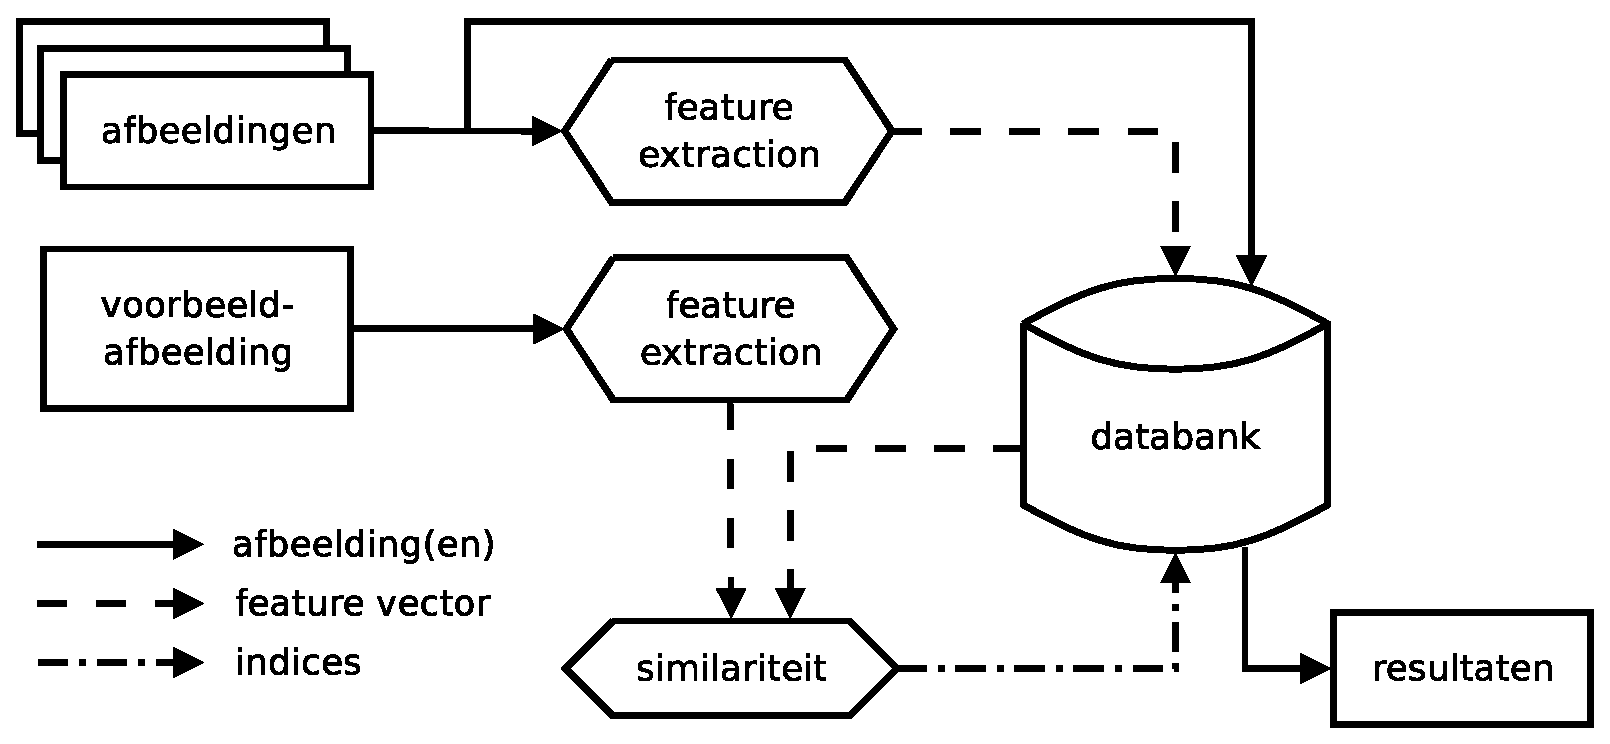
\includegraphics[width=\textwidth]{images/cbir.eps}
  \end{center}

  Terminologie: Content-Based Image Retrieval (CBIR).
}
\frame
{
  \frametitle{Similariteitsgebaseerd rangschikken van de zoekresultaten}
  
  Nadelen CBIR:
  \begin{itemize}
    \item Te complex voor zeer omvangrijke databanken.
    \item Gebruiker beschikt niet altijd over een geschikt voorbeeld.
  \end{itemize}

  Alternatief:
  \begin{center}
  \includegraphics[width=\textwidth]{images/simgeb_rangschikken.eps}
  \end{center}
  Extra laag bovenop TBIR die ervoor zorgt dat de resultaten gerangschikt
  worden volgens similariteit met een opgegeven verzameling van voorbeelden.
}

\section{Wiskundige fundamenten}
\frame
{
  \frametitle{Wiskundige fundamenten}

  Basisidee:
  \begin{enumerate}
  \item Beelden identificeren met \textbf{(L-)vaagverzamelingen}.
  \item Gebruik maken van \textbf{vaagsimilariteitsmaten} om de graduele 
  gelijkenis tussen dergelijke vaagverzamelingen te bepalen.
  \end{enumerate}
  
  \textbf{Aggregatieoperatoren} laten (onder andere) toe om
  \begin{itemize}
  \item componentsgewijs te werken
  \item en meerdere voorbeelden te ondersteunen.
  \end{itemize}
  
  \begin{opmerking}
  Notaties: $A^c = co_{N_s} A$, $A \cap B = A \cap_{T_M} B$, $A \cup B = A \cup_{S_M} B$,
  $A \setminus B = A \cap B^c$ en $A \triangle B = (A \setminus B) \cup (B \setminus A)$,
  met $A$ en $B$ vaagverzamelingen in een zelfde universum, $N_s$ de standaardnegator, 
  $T_M$ het minimum en $S_M$ het maximum.
  \end{opmerking}
}
\frame
{
  \frametitle{Ter herinnering}
  
  \begin{definitie}
  De \textbf{drager} van een vaagverzameling $A$ in $X$ wordt gedefinieerd als:
  \begin{minipage}{\textwidth}
  \vspace{6pt}
  \centering
  $\displaystyle supp\ A = \{x \in X \mid A(x) > 0\}$
  \end{minipage}
  \end{definitie}
%   \begin{definitie}
%   De \textbf{kern} van een vaagverzameling $A$ in $X$ wordt als volgt gedefinieerd:
%   \begin{displaymath}
%   ker\ A = \{x \in X \mid A(x) = 1\}
%   \end{displaymath}
%   \end{definitie}
  
  \vspace{10pt}
  Bij een eindige scherpe verzameling is de cardinaliteit het aantal 
  elementen in die verzameling. Dat concept kan als volgt uitgebreid 
  worden naar vaagverzamelingen:
  \begin{definitie}
  De \textbf{sigma count} van een vaagverzameling $A$ met eindige drager in een universum $X$, wordt
  gedefinieerd door:
  \begin{minipage}{\textwidth}
  \vspace{6pt}
  \centering
  $\displaystyle |A|=\sum_{x \in X} A(x)$
  \end{minipage}
  \end{definitie}
}

\section{Enkele begrippen uit beeldverwerking}
\frame
{
  \frametitle{Modellering van kleuren en beelden}

  \begin{definitie}
  Een tweedimensionaal \textbf{kleurbeeld} is een rooster dat bestaat uit een eindig aantal
  beeldpunten, die elk een bepaalde kleur hebben. 
  \end{definitie}
  
  \centering
  \begin{tabular}{@{}lr@{}}
  \begin{minipage}{0.7\textwidth}
  Modellering:
  \begin{itemize}
    \item Een \textbf{kleurmodel} is een abstract mathematisch model dat beschrijft
    hoe kleuren gerepresenteerd kunnen worden als $n$-tallen uit $\mathbb{R}^n$.
    Voorbeelden: RGB, HSV en L*a*b*.
    \item Als we de $n$-tallen uit het
    kleurmodel normaliseren tot $n$-tallen uit $[0,1]^n$, dan kunnen we een
    tweedimensionaal kleurbeeld modelleren als een $\mathbb{N}^2 - [0,1]^n$
    afbeelding.
%     $b$.
%     \item Voor een beeld $b$ van $M$ bij $N$ beeldpunten defini\"eren we de
%     $\mathbb{Z}^2 - [0,1]^n$ afbeelding $\mathring{b}$ als volgt:
%     \begin{displaymath}
%     \mathring{b}(x,y) = \begin{cases} 
%     b(x,y) & \text{als } 0 \le x < M \text{ en } 0 \le y < N \\
%     (0,0,\ldots,0) & \text{anders}
%     \end{cases}
%     \end{displaymath}
  \end{itemize}
  \end{minipage} &
  \begin{minipage}{0.3\textwidth}
  \centering
  \includegraphics[height=1.8cm]{images/rgb.eps}\\
  \includegraphics[height=1.8cm]{images/hsv.eps}\\[2pt]
  \includegraphics[height=1.8cm]{images/lab.eps}
  \end{minipage}
  \end{tabular}
}
\frame
{
  \frametitle{Kleurkwantisatie}
  
  De kleuren die op basis van een bepaald model kunnen voorgesteld worden, vormen
  een \textbf{kleurruimte}. Om de complexiteit te beperken is het vaak nodig om 
  het aantal kleuren in een kleurruimte te reduceren.
  
  \begin{definitie}
  Bij \textbf{kleurkwantisatie} wordt het aantal kleuren gereduceerd door 
  de kleuren te groeperen in zogenaamde \textbf{bins} en vervolgens alle kleuren van 
  een bin te vervangen door \'e\'en enkele kleur.
  \end{definitie}
  
  Modellering:
  \begin{itemize}
    \item De $C - \{1,2,\ldots,N\}$ afbeelding $bin$ associeert met elke kleur $c$, 
    uit een kleurruimte $C$, het nummer van de corresponderende bin.
    \item Met behulp van de $\{1,2,\ldots,N\} - C$ afbeelding $col$ kan de kleur van 
    elk van de $N$ bins bepaald worden.
  \end{itemize}
}
\frame
{
  \frametitle{Uniforme kwantisatie}
  
  \begin{flushleft}
  \begin{tabular}{@{}cc@{}}
  \begin{minipage}{0.65\textwidth}
  \begin{definitie}
  Bij \textbf{uniforme kwantisatie} wordt elke kleurcomponent uniform verdeeld
  in een aantal intervallen. De middelste waarden van de intervallen doen daarbij dienst
  als componenten van de kleur van een bin.
  \end{definitie}
  \end{minipage} &
  \begin{minipage}{0.3\textwidth}
  \centering
  \includegraphics[width=\textwidth]{images/flowers.eps}\\
  origineel
  \end{minipage}
  \end{tabular}
  \end{flushleft}
  We beschouwen zes manieren om uniform te kwantiseren, waarbij we telkens een ander
  kleurmodel gebruiken:
  \begin{center}
  \begin{tabular}{@{}c@{\ }c@{\ }c@{\ }c@{\ }c@{\ }c@{}}
  \includegraphics[width=0.15\textwidth]{images/uniform_hsv_flowers.eps} &
  \includegraphics[width=0.15\textwidth]{images/uniform_irb_flowers.eps} &
  \includegraphics[width=0.15\textwidth]{images/uniform_i1i2i3_flowers.eps} &
  \includegraphics[width=0.15\textwidth]{images/uniform_xyz_flowers.eps} &
  \includegraphics[width=0.15\textwidth]{images/uniform_yxy_flowers.eps} &
  \includegraphics[width=0.15\textwidth]{images/uniform_lab_flowers.eps} \\
  HSV & Irb & I1I2I3 & XYZ & Yxy & L*a*b* \\
  {\scriptsize $16 \cdot 4 \cdot 4$} & {\scriptsize $4 \cdot 8 \cdot 8$} & 
  {\scriptsize $4 \cdot 8 \cdot 8$} & {\scriptsize $8 \cdot 4 \cdot 8$} &
  {\scriptsize $4 \cdot 8 \cdot 8$} & {\scriptsize $4 \cdot 8 \cdot 8$}
  \end{tabular}
  \end{center}
}
\definecolor{zwart}{rgb}{0,0,0}
\definecolor{blauw}{rgb}{0,0,1}
\definecolor{groen}{rgb}{0,1,0}
\definecolor{rood}{rgb}{1,0,0}
\definecolor{bruin}{rgb}{0.5,0.16,0.16}
\definecolor{oranje}{rgb}{1,0.5,0}
\definecolor{geel}{rgb}{1,1,0}
\definecolor{paars}{rgb}{0.62,0.125,0.94}
\definecolor{grijs}{rgb}{0.75,0.75,0.75}
\definecolor{roze}{rgb}{1,0.75,0.79}
\definecolor{wit}{rgb}{1,1,1}
\frame
{
  \frametitle{Niet-uniforme kwantisatie}
  
  We beschouwen ook vier niet-uniforme kwantisatietechnieken:
  \begin{enumerate}
    \item \textbf{Smooth Color Transition (SCT) kwantisatie}: combinatie van twee uniforme
    kwantisaties, \'e\'en voor grijstinten en \'e\'en voor kleurtinten. Als 
    $s > 1 - 0.8\cdot v$ dan wordt de kleur benaderd met een kleurtint en anders met een
    grijstint.
    \item Mapping naar elf \textbf{focale kleuren} ({\color{zwart}zwart}, 
    {\color{blauw}blauw}, {\color{groen}groen}, {\color{rood}rood}, 
    {\color{bruin}bruin}, {\color{oranje}oranje}, {\color{geel}geel}, 
    {\color{paars}paars}, {\color{grijs}grijs}, {\color{roze}roze} en {\color{wit}wit}): 
    elke kleur vervangen door de focale kleur die het meest
    nabij licht in het perceptueel uniforme L*a*b*-model.
    \item \textbf{Neural Image Quantization (NeuQuant)}, waarbij gebruik gemaakt wordt van een 
    Kohonen neuraal netwerk.
    \item \textbf{Wu kwantisatie}, die gebaseerd is op dynamisch programmeren en principal 
    component analysis.
  \end{enumerate}
}
\frame
{
  \frametitle{Niet-uniforme kwantisatie}
  
  \begin{center}
  \begin{tabular}{@{}c@{\ }c@{\ }c@{\ }c@{\ }c@{\ }c@{}}
  \includegraphics[width=0.15\textwidth]{images/sct_flowers.eps} &
  \includegraphics[width=0.15\textwidth]{images/focal_flowers.eps} &
  \includegraphics[width=0.15\textwidth]{images/neuquant_flowers.eps} &
  \includegraphics[width=0.15\textwidth]{images/wu_flowers.eps} &
  \includegraphics[width=0.15\textwidth]{images/neuquant_flowers_8.eps} &
  \includegraphics[width=0.15\textwidth]{images/wu_flowers_8.eps} \\
  SCT & focaal & NeuQuant & Wu & NeuQuant & Wu \\
  {\scriptsize $256$} & {\scriptsize $256$} & 
  {\scriptsize $256$} & {\scriptsize $256$} &
  {\scriptsize $8$} & {\scriptsize $8$}
  \end{tabular}
  \end{center}
  Observaties:
  \begin{itemize}
  \item Onverwachte mapping bij focale kwantisatie:
  \begin{center}
  \includegraphics[height=2cm]{images/probleem_focale_kwantisatie.eps}
  \end{center}
  \item Wu kwantisatie is duidelijk meer geschikt dan NueQuant voor kwantisatie naar 
  een zeer klein aantal kleuren.
  \end{itemize}
}
\frame
{
  \frametitle{Kleurkwantisatie: rekentijd}
  
  \begin{center}
  \begin{minipage}[t]{0.45\textwidth}
  \vspace{0pt}
  \centering
  \includegraphics[height=2.85cm]{plots/uniform_quant_small_filled.eps}
  \end{minipage}
  \begin{minipage}[t]{0.45\textwidth}
  \vspace{0pt}
  \centering
  \includegraphics[height=3.1cm]{plots/neuquant_vs_wu_small_filled.eps}
  \end{minipage}
  \end{center}

  Observaties:
  \begin{itemize}
    \item Uniforme kwantisatie (naar 256 kleuren) is vaak sneller dan niet-uniforme.
    \item Wu kwantisatie is sneller dan NeuQuant, behalve voor een klein aantal kleuren.
  \end{itemize}
}
% \frame
% {
%   \frametitle{Lineaire filters}
% 
%   \begin{definitie}
%   Het beeld $b'$ dat we bekomen na toepassing van een \textbf{lineair filter} op 
%   een beeld $b$, wordt gegeven door de volgende correlatie:
%   \begin{minipage}{\textwidth}
%   \vspace{5pt}
%   \centering
%   $b'(x,y) = \displaystyle \sum_{(k,l) \in \Omega_m} \mathring{b}(x+k,y+l) \cdot m(k,l)$
%   \end{minipage}
%   met $\mathring{b}$ de nuluitbreiding van $b$, $m$ een $\mathbb{Z}^2 - \mathbb{R}$ 
%   afbeelding en $\Omega_m = \{ (k,l) \in \mathbb{Z}^2 \mid m(k,l) \ne 0 \}$.
%   %De functie $m$ wordt het \textbf{filtermasker} genoemd.
%   \end{definitie}
%   Voorbeeld: het 3x3 \textbf{binomiaalfilter}.
%   Voor het \textbf{filtermasker} $m_{bin}$ van dat filter geldt:
%   \begin{itemize} 
%     \item {\scriptsize $m_{bin}(-1,-1)=m_{bin}(-1,1)=m_{bin}(1,-1)=m_{bin}(1,1)=1/16$} 
%     \item {\scriptsize $m_{bin}(-1,0)=m_{bin}(0,-1)=m_{bin}(1,0)=m_{bin}(0,1)=1/8$}
%     \item {\scriptsize $m_{bin}(0,0)=1/4$}
%     \item {\scriptsize $m_{bin}(k,l)=0$ voor de overige $(k,l)$ uit $\mathbb{Z}^2$}
%   \end{itemize}
% }
% \frame
% {
%   \frametitle{Lineaire filters: binomiaalfilter}
%   
%   Als we veronderstellen dat $m_{bin}(k,l)=0$ voor alle posities
%   $(k,l)$ die niet weergegeven worden, dan kunnen we $m_{bin}$ noteren als
%   een matrix:
%   \begin{displaymath}
%   \scriptsize
%   \begin{array}{@{}l@{}}
%   \left[ \begin{array}{ccc} m_{bin}(-1,-1) & m_{bin}(0,-1) & m_{bin}(1,-1)\\ m_{bin}(-1,0) & m_{bin}(0,0) & m_{bin}(1,0)\\ m_{bin}(-1,1) & m_{bin}(0,1) & m_{bin}(1,1) \end{array} \right] \vspace{5pt}\\
%   \quad = \frac{1}{16}\left[ \begin{array}{ccc} 1 & 2 & 1\\ 2 & 4 & 2\\ 1 & 2 & 1 \end{array} \right]
%   = \frac{1}{16}\left[ \begin{array}{c} 1\\ 2\\ 1 \end{array} \right] \cdot 
%   \left[ \begin{array}{ccc} 1 & 2 & 1 \end{array} \right]
%   \end{array}
%   \end{displaymath}
% 
%   \begin{flushleft}
%   \begin{tabular}{@{}lr@{}}
%   \begin{minipage}{0.3\textwidth}
%   \begin{tabular}{@{}l@{}}
%   $\begin{array}{@{}c@{}}
%   1 \\
%   1\quad 1 \\	
%   \textbf{1}\quad \textbf{2}\quad \textbf{1} \\
%   1\quad 3\quad 3\quad 1 \\ 
%   1\quad 4\quad 6\quad 4\quad 1
%   \end{array}$ \vspace{5pt}\\
%   {\scriptsize driehoek van Pascal}
%   \end{tabular}
%   \end{minipage} &
%   \begin{minipage}{0.65\textwidth}
%   Meer algemeen kan het $N$x$N$ binomiaalfilter geschreven worden als de matrix $R^T \cdot R$,
%   waarbij: 
%   \begin{displaymath}
%   R=2^{-N+1} \cdot \left[ \begin{array}{cccc} \binom{N-1}{0} & \binom{N-1}{1} & 
%   \ldots & \binom{N-1}{N-1} \end{array} \right]
%   \end{displaymath}
%   \end{minipage}
%   \end{tabular}
%   \end{flushleft}
% }
% \frame
% {
%   \frametitle{Eenvoudige randdetectie}
%   
%   In een tweedimensionaal beeld $b$ zijn randen plaatsen waar de luminantiecomponent
%   $lum(x,y)$ van $b(x,y)$ sterk varieert als funtie van $x$ en/of $y$. Bijgevolg
%   kunnen we een formule op basis van de \textbf{gradi\"ent} gebruiken om randen te 
%   detecteren in $b$:
%   \begin{displaymath}
%   |\nabla lum(x,y)| / \sqrt{2} = \sqrt{(D_1 lum(x,y))^2 + (D_2 lum(x,y))^2} / \sqrt{2}
%   \end{displaymath}
%   Discrete benadering van partieel afgeleiden van $lum$:
%   \begin{displaymath}
%   \begin{array}{c}
%   D_1 lum(x,y) \approx \frac{lum(x+1,y) - lum(x-1,y)}{2}\vspace{4pt}\\
%   D_2 lum(x,y) \approx \frac{lum(x,y+1) - lum(x,y-1)}{2}
%   \end{array}
%   \end{displaymath}
%   Met lineaire filters:
%   \begin{displaymath}
%   \scriptsize
%   D_1 lum(x,y)\text{: } \frac{1}{2} \left[ \begin{array}{@{\ }ccc@{\ }} -1 & 0 & 1 \end{array} \right] \text{, } 
%   D_2 lum(x,y)\text{: } \frac{1}{2} \left[ \begin{array}{@{\ }c@{\ }} -1 \\ 0 \\ 1 \end{array} \right]
%   \end{displaymath}
% }
% \frame
% {
%   \frametitle{Eenvoudige randdetectie}
%   
%   \textbf{Sobel-operator}: variant op gradi\"entmethode met extra ruisonderdrukking
%   door binomiaalfilter loodrecht op de richting van de parti\"ele afleiding:
%   \begin{displaymath}
%   \scriptsize
%   D_1 lum(x,y)\text{: } \frac{1}{8} \left[ \begin{array}{@{\ }c@{\ }} 1 \\ 2 \\ 1 \end{array} \right] \cdot \left[ \begin{array}{@{\ }ccc@{\ }} -1 & 0 & 1 \end{array} \right] \text{, } 
%   D_2 lum(x,y)\text{: } \frac{1}{8} \left[ \begin{array}{@{\ }c@{\ }} -1 \\ 0 \\ 1 \end{array} \right] \cdot \left[ \begin{array}{@{\ }ccc@{\ }} 1 & 2 & 1 \end{array} \right]
%   \end{displaymath}
%   Geen spectaculair verschillende resultaten:
%   \begin{center}
%   \begin{tabular}{@{}c@{\ }c@{\ }c@{}}
%   \includegraphics[width=0.3\textwidth]{images/lena_met_ruis.eps} &
%   \includegraphics[width=0.3\textwidth]{images/edges_lena_met_ruis.eps} &
%   \includegraphics[width=0.3\textwidth]{images/edges_sobel_lena_met_ruis.eps}\\
%   {\scriptsize ruizig luminantiebeeld} & {\scriptsize gradi\"ent} & {\scriptsize Sobel}
%   \end{tabular}
%   \end{center}
% }

\section{Similariteitsmaten voor beelden}
\frame
{
  \frametitle{Definitie en eigenschappen}

  \begin{definitie}
  Een \textbf{similariteitsmaat voor beelden} is een maat die de gelijkenis 
  tussen twee gegeven beelden uitdrukt als een getal in het eenheidsinterval 
  $[0,1]$.
  \end{definitie}

  Eigenschappen:
  \begin{itemize}
  \item Reflexief: $M(A,A)=1$
  \item Symmetrisch: $M(A,B)=M(B,A)$
  \item Geen (vorm van) transitiviteit, want dat zou bijvoorbeeld impliceren dat 
  het eerste en het laatste beeld van
  \begin{center}
  \vspace{5pt}
  \includegraphics[width=1cm]{images/video_trans_1.eps}\ 
  \includegraphics[width=1cm]{images/video_trans_2.eps}\ 
  \includegraphics[width=1cm]{images/video_trans_3.eps}\ 
  \includegraphics[width=1cm]{images/video_trans_4.eps}\ 
  \includegraphics[width=1cm]{images/video_trans_5.eps}\
  \includegraphics[width=1cm]{images/video_trans_6.eps}\ 
  \ldots\ 
  \includegraphics[width=1cm]{images/video_trans_10.eps}\ 
  \includegraphics[width=1cm]{images/video_trans_11.eps}
  \end{center}
  zeer similair zijn, wat niet overeenkomt met onze intu\"itie.
  \end{itemize}
}
\frame
{
  \frametitle{Constructie}
  
  We kunnen een similariteitsmaat voor beelden construeren door:
  \begin{enumerate}
    \item elk mogelijk beeld, al dan niet rechtstreeks, te identificeren
    met een (L-)vaagverzameling.
    \item gebruik te maken van vaagsimilariteitsmaten om die (L-)vaagverzamelingen
    te vergelijken.
  \end{enumerate}
  
  \begin{opmerking}
  In het vervolg bedoelen we met ``similariteitsmaat'' steeds
  de combinatie van een vaagsimilariteitsmaat met een manier om beelden te 
  identificeren met vaagverzamelingen. Dus: 
  \begin{itemize}
    \item ``similariteitsmaat'' $\neq$ een vaagsimilariteitsmaat op zich
    \item ``similariteitsmaat'' $=$ een similariteitsmaat voor beelden op basis van een vaagsimilariteitsmaat
  \end{itemize}
  \end{opmerking}
}
\frame
{
  \frametitle{Evaluatie van performantie: testcollectie}

  Testcollectie van $N$ beelden die corresponderen met 
  $N/N_R$ objecten die elk $N_R$ keer gefotografeerd werden:

\begin{center}

\begin{tabular}{c@{\ }c@{}c@{}c@{}c@{}c c@{\ }c@{}c@{}c@{}c@{}c}

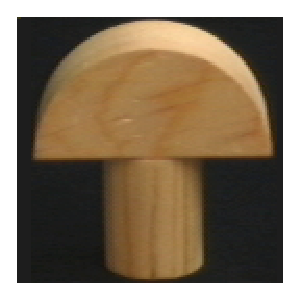
\includegraphics[width=0.8cm]{coil/beeld-0.eps} &
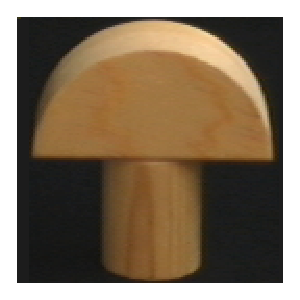
\includegraphics[width=0.8cm]{coil/beeld-1.eps} &
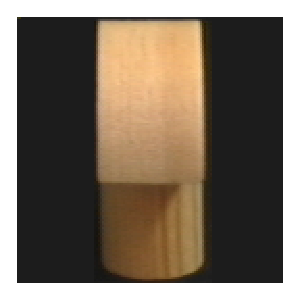
\includegraphics[width=0.8cm]{coil/beeld-2.eps} &
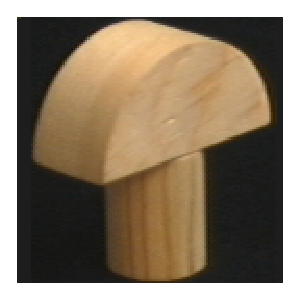
\includegraphics[width=0.8cm]{coil/beeld-3.eps} &
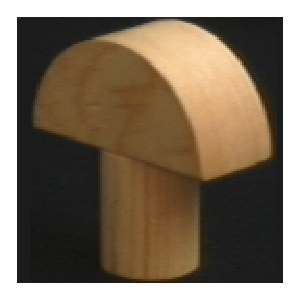
\includegraphics[width=0.8cm]{coil/beeld-4.eps} &
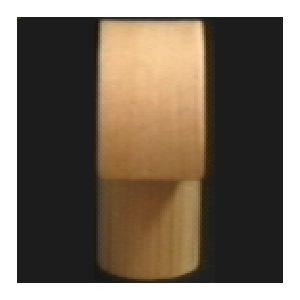
\includegraphics[width=0.8cm]{coil/beeld-5.eps} &

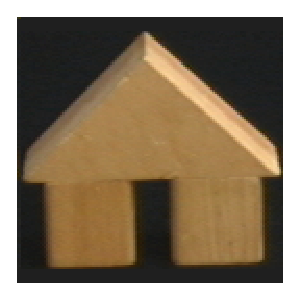
\includegraphics[width=0.8cm]{coil/beeld-42.eps} &
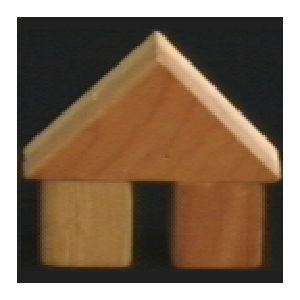
\includegraphics[width=0.8cm]{coil/beeld-43.eps} &
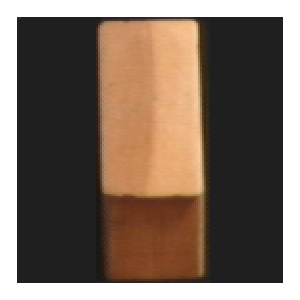
\includegraphics[width=0.8cm]{coil/beeld-44.eps} &
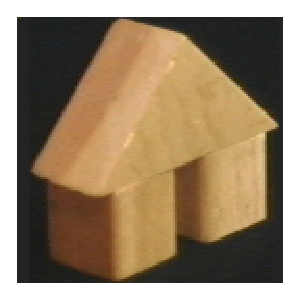
\includegraphics[width=0.8cm]{coil/beeld-45.eps} &
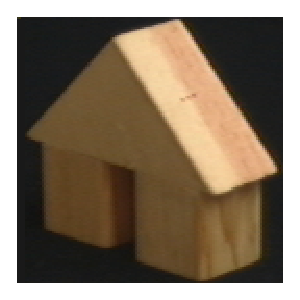
\includegraphics[width=0.8cm]{coil/beeld-46.eps} &
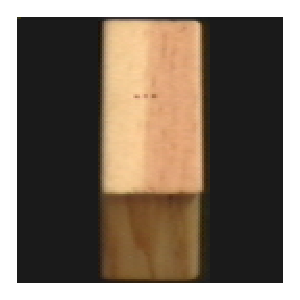
\includegraphics[width=0.8cm]{coil/beeld-47.eps} \\

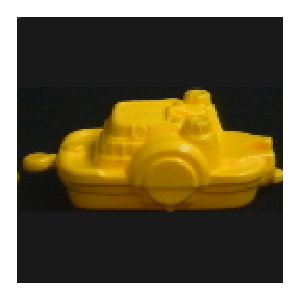
\includegraphics[width=0.8cm]{coil/beeld-12.eps} &
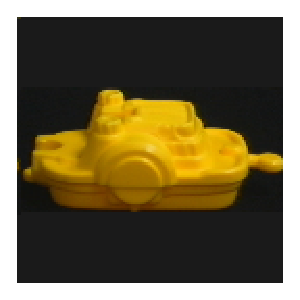
\includegraphics[width=0.8cm]{coil/beeld-13.eps} &
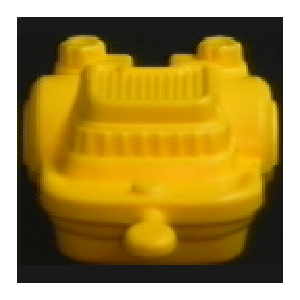
\includegraphics[width=0.8cm]{coil/beeld-14.eps} &
\includegraphics[width=0.8cm]{coil/beeld-15.eps} &
\includegraphics[width=0.8cm]{coil/beeld-16.eps} &
\includegraphics[width=0.8cm]{coil/beeld-17.eps} &

\includegraphics[width=0.8cm]{coil/beeld-18.eps} &
\includegraphics[width=0.8cm]{coil/beeld-19.eps} &
\includegraphics[width=0.8cm]{coil/beeld-20.eps} &
\includegraphics[width=0.8cm]{coil/beeld-21.eps} &
\includegraphics[width=0.8cm]{coil/beeld-22.eps} &
\includegraphics[width=0.8cm]{coil/beeld-23.eps} \\

\includegraphics[width=0.8cm]{coil/beeld-24.eps} &
\includegraphics[width=0.8cm]{coil/beeld-25.eps} &
\includegraphics[width=0.8cm]{coil/beeld-26.eps} &
\includegraphics[width=0.8cm]{coil/beeld-27.eps} &
\includegraphics[width=0.8cm]{coil/beeld-28.eps} &
\includegraphics[width=0.8cm]{coil/beeld-29.eps} &

\includegraphics[width=0.8cm]{coil/beeld-54.eps} &
\includegraphics[width=0.8cm]{coil/beeld-55.eps} &
\includegraphics[width=0.8cm]{coil/beeld-56.eps} &
\includegraphics[width=0.8cm]{coil/beeld-57.eps} &
\includegraphics[width=0.8cm]{coil/beeld-58.eps} &
\includegraphics[width=0.8cm]{coil/beeld-59.eps} \\

\includegraphics[width=0.8cm]{coil/beeld-30.eps} &
\includegraphics[width=0.8cm]{coil/beeld-31.eps} &
\includegraphics[width=0.8cm]{coil/beeld-32.eps} &
\includegraphics[width=0.8cm]{coil/beeld-33.eps} &
\includegraphics[width=0.8cm]{coil/beeld-34.eps} &
\includegraphics[width=0.8cm]{coil/beeld-35.eps} &

\includegraphics[width=0.8cm]{coil/beeld-36.eps} &
\includegraphics[width=0.8cm]{coil/beeld-37.eps} &
\includegraphics[width=0.8cm]{coil/beeld-38.eps} &
\includegraphics[width=0.8cm]{coil/beeld-39.eps} &
\includegraphics[width=0.8cm]{coil/beeld-40.eps} &
\includegraphics[width=0.8cm]{coil/beeld-41.eps} \\

\includegraphics[width=0.8cm]{coil/beeld-6.eps} &
\includegraphics[width=0.8cm]{coil/beeld-7.eps} &
\includegraphics[width=0.8cm]{coil/beeld-8.eps} &
\includegraphics[width=0.8cm]{coil/beeld-9.eps} &
\includegraphics[width=0.8cm]{coil/beeld-10.eps} &
\includegraphics[width=0.8cm]{coil/beeld-11.eps} &

\includegraphics[width=0.8cm]{coil/beeld-48.eps} &
\includegraphics[width=0.8cm]{coil/beeld-49.eps} &
\includegraphics[width=0.8cm]{coil/beeld-50.eps} &
\includegraphics[width=0.8cm]{coil/beeld-51.eps} &
\includegraphics[width=0.8cm]{coil/beeld-52.eps} &
\includegraphics[width=0.8cm]{coil/beeld-53.eps} \\

\includegraphics[width=0.8cm]{coil/beeld-60.eps} &
\includegraphics[width=0.8cm]{coil/beeld-61.eps} &
\includegraphics[width=0.8cm]{coil/beeld-62.eps} &
\includegraphics[width=0.8cm]{coil/beeld-63.eps} &
\includegraphics[width=0.8cm]{coil/beeld-64.eps} &
\includegraphics[width=0.8cm]{coil/beeld-65.eps} &
\multicolumn{2}{c}{$N_R = 6$} & 
\multicolumn{4}{c}{$N = 11 \cdot N_R = 66$}

\end{tabular}
\end{center}

}
\frame
{
  \frametitle{Evaluatie van performantie: GGR}

  We gebruiken de te evalueren similariteitsmaat om de testcollectie te rangschikken 
  volgens similariteit met een voorbeeld. Beschouw nu de vector 
  $(r_1,r_2,\ldots,r_{N_R}) \in \{1,2,\ldots,N\}^{N_R}$, 
  waarbij $r_i$ het rangnummer van het $i$-de relevante beeld voorstelt.

  \begin{definitie}
  
  De \textbf{genormaliseerde gemiddelde rang} (GGR) wordt gegeven door de volgende afbeelding:
  $$
  \small\begin{array}{lrcl}
  \text{GGR}: & \{1,2,\ldots,N\}^{N_R} & \to 	& [0,1] \\
		& (r_1,r_2,\ldots,r_{N_R}) & \mapsto &
	{\displaystyle\frac{1}{N \cdot N_R}\left[ \left(\sum_{i=1}^{N_R}r_i\right) - \frac{N_R \cdot (N_R + 1)}{2} \right]},\\[15pt]
	& & & \qquad \quad \forall (r_1, r_2, ..., r_{N_R}) \in \{1,2,\ldots,N\}^{N_R}
  \end{array}
  $$
  \end{definitie}
 
  De GGR nadert naar $1$ naarmate de performantie slechter wordt.
}
\frame
{
  \frametitle{Evaluatie van performantie: GGGR}

  \begin{description}
  \item[Probleem:] De GGR kan een verkeerd beeld geven omdat de performantie afhankelijk
  kan zijn van het gekozen voorbeeld. 
  \item[Oplossing:]
  We berekenen de GGR voor
  \begin{center}
  \vspace{5pt}
  \includegraphics[width=0.8cm]{coil/beeld-0.eps}, 
  \includegraphics[width=0.8cm]{coil/beeld-42.eps}, 
  \includegraphics[width=0.8cm]{coil/beeld-12.eps}, 
  \includegraphics[width=0.8cm]{coil/beeld-18.eps}, 
  \includegraphics[width=0.8cm]{coil/beeld-24.eps}, 
  \includegraphics[width=0.8cm]{coil/beeld-54.eps},\\
  \vspace{5pt}
  \includegraphics[width=0.8cm]{coil/beeld-30.eps}, 
  \includegraphics[width=0.8cm]{coil/beeld-36.eps}, 
  \includegraphics[width=0.8cm]{coil/beeld-6.eps}, 
  \includegraphics[width=0.8cm]{coil/beeld-48.eps}\ en  
  \includegraphics[width=0.8cm]{coil/beeld-60.eps}, 
  \end{center}
  en we beschouwen het gemiddelde van de bekomen waarden. 
  De waarde die we zo bekomen noemen we de
  \textbf{globale genormaliseerde gemiddelde rang} (GGGR).
  \end{description}
}
\frame
{
  \frametitle{Evaluatie van performantie: rekentijd}
  
  We meten ook hoe lang het duurt om de rangschikkingen, die nodig zijn om 
  de GGGR te bepalen, te berekenen. Voor onze praktische implementatie
  is de rekentijd echter minder belangrijk dan de GGGR, want:
  \begin{itemize}
    \item De collecties van beelden waarop de similariteitsmaten toegepast worden,
    zijn beperkt in grootte.
    \item Het uivoeren van de berekeningen gebeurd aan de kant van de client, 
    waardoor er geen gevaar is voor overbelasting van de server.
  \end{itemize}
  Bij echte CBIR:
  \begin{itemize}
    \item is de rekentijd wel cruciaal,
    \item maar het is wel mogelijk om berekeningen op voorhand te doen en de resultaten
    ervan samen met de beelden op te slaan in de databank.
  \end{itemize}
}
\frame
{
  \frametitle{Beperken rekentijd}
  
  Stel dat $A$ en $B$ twee vaagverzamelingen zijn in een zelfde universum $X$. 
  Als $X'= supp\ A \cup supp\ B$ veel minder elementen bevat dan $X$, dan kunnen we 
  de rekentijd sterk reduceren door het bereik van de sommaties in de 
  vaagsimilariteitsmaten te beperken tot $X'$. Wanneer we $||C|| = \sum_{x \in X'} C(x)$
  defini\"eren voor elke $C \in \mathcal{F}_L(X)$, dan vinden we bijvoorbeeld:
  \begin{align*}
  \scriptstyle M_{7c}(A,B) 
  & \scriptstyle\ = \displaystyle \frac{\scriptstyle |A^c \cap B^c|}{\scriptstyle \max \{|A^c|,|B^c|\}} & & {\scriptsize \scriptstyle \text{definitie } M_{7c}} \\
  & \scriptstyle\ = \displaystyle \frac{\scriptstyle |X|-|A \cup B|}{\scriptstyle \max \{|X|-|A|,|X|-|B|\}} & & {\scriptsize \scriptstyle (\forall C \in \mathcal{F}_L(X))(|C^c|=|X|-|C|)} \\ 
  & \scriptstyle\ = \displaystyle \frac{\scriptstyle |X|-||A \cup B||}{\scriptstyle \max \{|X|-||A||,|X|-||B||\}} & & {\scriptsize \scriptstyle |A \cup B|=||A \cup B|| \text{, } |A|=||A|| \text{ en } |B|=||B||} \\
  & \scriptstyle\ = \displaystyle \frac{\scriptstyle |X|-||A \cup B||}{\scriptstyle |X| - \min \{||A||,||B||\}} & & {\scriptsize \scriptstyle (\forall (a,b,c) \in \mathbb{R}^3)(\max\{c-a,c-b\}=c-\min\{a,b\})}
  \end{align*}
}
\frame
{
  \frametitle{Beperken rekentijd}

  \begin{minipage}{\textwidth}
  \centering
  \scriptsize
  \begin{tabular}{@{}ccc@{}}
  $M_{7}(A,B) = \displaystyle \frac{|A \cap B|}{\max \{|A|,|B|\}}$ & $\displaystyle\to$ &
  $M_{7}(A,B) = \displaystyle \frac{||A \cap B||}{\max \{||A||,||B||\}}$ \vspace{5pt}\\
  \begin{tabular}{r}
  $|X|+1$ vergelijkingen\\
  $3\cdot (|X|-1)$ optellingen\\
  $1$ deling\\
  \hline
  $4\cdot |X| - 1$
  \end{tabular} & &
  \begin{tabular}{r}
  $|X'|+1$ vergelijkingen\\ 
  $3\cdot (|X'|-1)$ optellingen\\
  $1$ deling\\
  \hline
  $4\cdot |X'| - 1$
  \end{tabular} 
  \end{tabular}
  \vspace{4pt}
  \end{minipage}
  Als $|X'| \ll |X|$ dan is de herschreven vorm inderdaad een stuk sneller.
  
  \begin{minipage}{\textwidth}
  \vspace{4pt}
  \centering
  \scriptsize
  \begin{tabular}{@{}ccc@{}}
  $M_{7c}(A,B) = \displaystyle \frac{|A^c \cap B^c|}{\max \{|A^c|,|B^c|\}}$ & $\displaystyle\to$ &
  $M_{7c}(A,B) = \displaystyle \frac{|X|-||A \cup B||}{|X| - \min \{||A||,||B||\}}$ \vspace{5pt}\\
  \begin{tabular}{r}
  $|X|+1$ vergelijkingen\\
  $3\cdot (|X|-1)$ optellingen\\
  $1$ deling\\
  $2\cdot |X|$ aftrekkingen\\
  \hline
  $6\cdot |X| - 1$
  \end{tabular} & &
  \begin{tabular}{r}
  $|X'|+1$ vergelijkingen\\
  $3\cdot (|X'|-1)$ optellingen\\
  $1$ deling\\
  $2$ aftrekkingen\\
  \hline
  $4\cdot |X'| + 1$
  \end{tabular}
  \end{tabular} 
  \vspace{4pt}
  \end{minipage} 
  Zelfs voor $|X'|=|X|$ zal $4\cdot |X'| + 1$ doorgaans kleiner zijn dan
  $6\cdot |X| - 1$. Als $|X'| \ll |X|$ dan wordt het verschil in rekentijd uiteraard
  nog significanter.
}

\section{Pixelgebaseerde similariteitsmaten}
\frame
{
  \frametitle{Pixelgebaseerde similariteitsmaten voor grijswaardebeelden}
%   \begin{definitie}
%   Een tweedimentionaal \textbf{binair beeld} is een eindig rooster dat enkel 
%   witte en zwarte beeldpunten bevat.
%   \end{definitie}
%   Representatie: scherpe verzameling $A$ in $\mathbb{N}^2$ met:
%   \begin{displaymath}
%   \begin{array}{rcl}
%   p \in A & \iff & p \text{ is een wit punt in het beeld} \\
%   p \notin A & \iff & p \text{ is een zwart punt in het beeld}
%   \end{array}
%   \end{displaymath}
  \begin{definitie}
  Een tweedimensionaal \textbf{grijswaardebeeld} is een eindig rooster dat
  naast wit en zwart ook grijstinten kan bevatten.
  \end{definitie}
  Representatie: een vaagverzameling $A$ in $\mathbb{N}^2$ bepaald door:
  \begin{displaymath}
  \begin{array}{rcl}
  A(p) = 1 & \iff & p \text{ is een wit punt in het beeld} \\
  A(p) = 0 & \iff & p \text{ is een zwart punt in het beeld} \\
  A(p) \in\ ]0,1[ & \iff & p \text{ is een beeldpunt met een grijstint}
  \end{array}
  \end{displaymath}
  Daarbij geldt: hoe groter de grijswaarde, hoe lichter de grijstint.
  
  \begin{flushleft}
  Door de bovenstaande representatie te combineren met een vaagsimilariteitsmaat,
  bekomen we een similariteitsmaat voor grijswaardebeelden. Omdat het universum
  daarbij bestaat uit beeldpunten (pixels), spreken we van
  \textbf{pixelgebaseerde} similariteitsmaten.
  \end{flushleft}
}
\frame
{
  \frametitle{Pixelgebaseerde similariteitsmaten voor kleurbeelden}
  
  \begin{description}
     \item[Probleem:] De meeste beelden op internet zijn 
     geen grijswaardebeelden maar kleurbeelden.
     \item[Oplossing:] We beschouwen drie mogelijke oplossingen:
     \begin{enumerate}
       \item Beelden eerst omzetten naar grijswaardebeelden, bijvoorbeeld aan de 
       hand van de formule $0.3 \cdot r + 0.59 \cdot g + 0.11 \cdot b$.
       \item Een similariteitsmaat voor grijswaardebeelden toepassen op elke
       kleurcomponent en vervolgens de resultaten voor de verschillende componenten
       aggregeren tot \'e\'en getal.
       \item Een traliegebaseerde representatie voor kleurbeelden defini\"eren (zie
       volgende slide).
     \end{enumerate}
   \end{description}
}
\frame
{
  \frametitle{Pixelgebaseerde similariteitsmaten voor kleurbeelden}

  Traliegebaseerde aanpak: in het geval van het RGB-model kunnen kleurbeelden 
  gerepresenteerd worden door een L-vaagverzameling in $\mathbb{N}^2$,
  waarbij we de complete tralie $([0,1]^3, \le_{RGB,lex})$ gebruiken:
  \begin{minipage}{\textwidth}
  \vspace{7pt}
  \small
  \centering
  $\begin{array}{@{}r@{}l@{}}
   c <_{RGB} c' & \ \iff d(c,Bl) < d(c',Bl)\ \lor \\
			 & \ \qquad \qquad (d(c,Bl) = d(c',Bl) \land d(c,Wh) > d(c',Wh)) \\[4pt]
   c >_{RGB} c' & \ \iff d(c,Wh) < d(c',Wh)\ \lor \\
			 & \ \qquad \qquad (d(c,Wh) = d(c',Wh) \land d(c,Bl) > d(c',Bl)) \\[4pt]
   c =_{RGB} c' & \ \iff (d(c,Bl) = d(c',Bl) \land d(c,Wh) = d(c',Wh)) \\[4pt]
   c \leq_{lex} c' & \ \iff r < r' \lor (r = r' \land g < g')\ \lor \\
   			 & \ \qquad \qquad (r = r' \land g = g' \land b \leq b') \\[4pt]
   c \leq_{RGB,lex} c' & \ \iff c <_{RGB} c' \lor (c =_{RGB} c' \land c \leq_{lex} c')
  \end{array}$
  \vspace{7pt}
  \end{minipage}
  met $Bl = (0,0,0)$, $Wh = (1,1,1)$ en $d$ de Euclidische afstand.
}
\frame
{ 
  \frametitle{Pixelgebaseerde similariteitsmaten voor kleurbeelden}

  Voor de traliegebaseerde aanpak moeten de bewerkingen waarvan de 
  vaagsimilariteitsmaten gebruik maken, veralgemeend worden van 
  $[0,1]$ naar $[0,1]^3$. We gebruiken $c - c' = (r-r',g-g',b-b')$, 
  $|c| = \frac{1}{\sqrt{3}} \cdot \sqrt{r^2 + g^2 + b^2}$, $1 - c = (1,1,1) - (r,g,b)$ en:
  \begin{minipage}{\textwidth}
    \vspace{4pt}
    \scriptsize
    \centering
%     $c - c' = (r-r',g-g',b-b')$ \  
%     $|c| = \frac{1}{\sqrt{3}} \cdot \sqrt{r^2 + g^2 + b^2}$\ 
%     $1 - c = (1,1,1) - (r,g,b)$\\
    $\min \{c,c'\} = \begin{cases}
    c & \text{als } c <_{RGB} c' \lor (c =_{RGB} c' \land c \leq_{lex} c') \\
    c' & \text{anders}
    \end{cases}$\\[2pt]
    $\max \{c,c'\} = \begin{cases}
    c' & \text{als } c <_{RGB} c' \lor (c =_{RGB} c' \land c \leq_{lex} c') \\
    c & \text{anders}
    \end{cases}$
    \vspace{4pt}
  \end{minipage}
  voor elke $c(r,g,b),c'(r',g',b') \in [0,1]^3$. 
  Het begrip sigma count veralgemenen we als volgt:
  \begin{minipage}{\textwidth}
  \vspace{4pt}
  \scriptsize
  \centering
  $\displaystyle |A|=\frac{1}{\sqrt{3}}\sum_{p \in P}\sqrt{(A_1(p))^2+(A_2(p))^2+(A_3(p))^2}$
  \vspace{4pt}
  \end{minipage}
  met $A(p)=(A_1(p),A_2(p),A_3(p))$ voor alle $p$ uit het
  universum der beeldpunten $P$.
}
\frame
{
  \frametitle{Resolutie-onafhankelijke similariteitsmaten}
  
  \begin{definitie}
  Het aantal pixels in een beeld wordt de \textbf{resolutie} van dat beeld genoemd.
  \end{definitie}
  \begin{description}
	\item[Probleem:] De similariteitsmaten die we tot nu toe beschouwd hebben, kunnen
	enkel toegepast worden op beelden die dezelfde resolutie hebben.
	\item[Oplossing:] Constructie van resolutie-onafhankelijke 
	pixelgebaseerde similariteitsmaten door
	\begin{itemize}
      \item \textbf{intermediaire beelden} of 
      \item \textbf{beeldonderdelen} 
    \end{itemize}
    te beschouwen.
  \end{description}
}
\frame
{
  \frametitle{Resolutie-onafhankelijke similariteitsmaten: intermediaire beelden}

  \begin{center}
  \begin{tabular}{@{}lc@{}}
  \begin{minipage}{0.6\textwidth}
  De beelden \textbf{herschalen} zodanig dat we twee beelden met dezelfde resolutie bekomen. 
  \end{minipage} & 
  \begin{minipage}{0.4\textwidth}
  \includegraphics[height=0.25\textheight]{images/rescale.eps}
  \end{minipage}\vspace{5pt}\\
  \begin{minipage}{0.6\textwidth}
  Eerst \textbf{kleurkwantisatie} met een variabel kleurenpalet toepassen en vervolgens een
  nieuw beeld construeren op basis van de kleuren van het bekomen palet.
  \end{minipage} &
  \begin{minipage}{0.4\textwidth}
  \includegraphics[height=0.25\textheight]{images/dominant_colors.eps}
  \end{minipage}\vspace{5pt}\\
  \begin{minipage}{0.6\textwidth}
  \textbf{Kleurmomenten} (gemiddelde, variantie en scheefheid) gebruiken om nieuwe 
  intermediaire beelden te construeren.
  \end{minipage} &
  \begin{minipage}{0.4\textwidth}
  \includegraphics[height=0.25\textheight]{images/moments.eps}
  \end{minipage}
  \end{tabular}
  \end{center}
}
\frame
{
  \frametitle{Resolutie-onafhankelijke similariteitsmaten: beeldonderdelen}
  
  \begin{minipage}{\textwidth}
  \centering
  \includegraphics[width=0.65\textwidth]{images/multires.eps}\qquad
  \includegraphics[width=0.25\textwidth]{images/multires_sim-matrix_beide.eps}
  \vspace{4pt}
  \end{minipage}
  Ruwe schets van werking:
  \begin{enumerate}
    \item Beelden partitioneren in beeldonderdelen met dezelfde resolutie 
    ($8 \cdot 8$ pixels).
    \item De beeldonderdelen (van groot naar klein) ordenen op basis van
    hun gemiddelde kleur, met behulp van $\le_{RGB,lex}$.
    \item Gebruik maken van de ordening om grote similariteiten te vinden.
    \item Het gemiddelde van de grote similariteiten bepalen.
  \end{enumerate}
}
\frame
{
  \frametitle{Experimentele observaties}
  
  %De GGGR-waarde en de rekentijd in ms voor elk van de similariteitsmaten op basis 
  %van herschaalde beelden:
  \begin{center}
  \begin{tabular}{@{}c@{}c@{}}
  \includegraphics[width=0.5\textwidth]{plots/scaling_gggrs_en_cputimes_filled.eps} &
  \includegraphics[width=0.5\textwidth]{plots/moments_gggrs_en_cputimes_filled.eps}\\
  {\scriptsize intermediaire beelden: herschaling} & {\scriptsize intermediaire beelden: kleurmomenten} \vspace{10pt}\\
  \includegraphics[width=0.5\textwidth]{plots/dom_colors_neuquant_gggrs_en_cputimes_filled.eps} &
  \includegraphics[width=0.5\textwidth]{plots/dom_colors_wu_gggrs_en_cputimes_filled.eps}\\
  {\scriptsize intermediaire beelden: NeuQuant} & {\scriptsize intermediaire beelden: Wu}
  \end{tabular}
  \end{center}
}
\frame
{
  \frametitle{Experimentele observaties}
  
  \begin{center}
  \begin{tabular}{@{}cc@{}}
  \begin{minipage}{0.5\textwidth}
  \begin{tabular}{@{}c@{}}
  \includegraphics[width=\textwidth]{plots/multires_gggrs_en_cputimes_filled.eps}\\
  {\scriptsize beeldonderdelen}
  \end{tabular}
  \end{minipage} &
  \begin{minipage}{0.4\textwidth}
  \raggedright
  De gegevens in de onderstaande tabel werden berekend uit de GGGRs van alle 
  pixelgebaseerde similariteitsmaten die we beschouwd hebben.
  \end{minipage} \vspace{10pt}
  \end{tabular}
  \end{center}

  \begin{center}
  \tiny
  \begin{tabular}{r|cccccccc}
  & $M_{1a}$ & $M_{1b}$ & $M_{1c}$ & $M_{2}$ & $M_{3}$ & $M_{5}$ & $M_{5c}$ & $M_{6}$ \\
  \hline
  minimale GGGR & 0.0147 & 0.0245 & 0.0323 & 0.0355 & 0.0093 & 0.0128 & 0.0219 & 0.0102 \\
  gemiddelde GGGR & 0.0818 & 0.0951 & 0.1115 & 0.1428 & {\color{white} 0.0802} & 0.0922 & 0.0971 & 0.1024\vspace{8pt}\\
  & $M_{6c}$ & $M_{7}$ & $M_{7c}$ & $M_{8}$ & $M_{8c}$ & $M_{9}$ & $M_{9c}$ & $M_{10}$ \\
  \hline
  minimale GGGR & 0.0212 & 0.0089 & 0.0203 & 0.2024 & 0.1985 & {\color{white} 0.0084} & 0.0201 & 0.2212 \\
  gemiddelde GGGR & 0.1145 & 0.0873 & 0.0922 & 0.3604 & 0.3688 & 0.0806 & 0.0868 & 0.3895\vspace{8pt}\\
  & $M_{10c}$ & $M_{11}$ & $M_{11c}$ & $M_{12}$ & $M_{13}$ & $M_{I_3}$ & $M_{I_{3c}}$ \\
  \hline
  minimale GGGR & 0.2106 & 0.0128 & 0.0219 & 0.0203 & 0.1985 & 0.0102 & 0.0212 \\
  gemiddelde GGGR & 0.3850 & 0.0922 & 0.0971 & 0.0922 & 0.3696 & 0.1035 & 0.1038
  \end{tabular}
  \end{center} 
}
\frame
{
  \frametitle{Experimentele observaties}
  
%   Tot nu toe hebben we telkens het gemiddelde gebruikt om te aggregeren bij
%   de componentsgewijze aanpak. We kunnen echter ook een t-norm gebruiken.
%   De beelden kunnen dan enkel similair 
%   zijn indien \emph{alle} kleurcomponenten goed op elkaar lijken.
  
  Aggregeren met een t-norm (in plaats van het gemiddelde) bij de componentsgewijze 
  aanpak: beelden kunnen enkel similair zijn indien \emph{alle} kleurcomponenten 
  goed op elkaar lijken.
  
  \begin{center}
  \begin{tabular}{@{}c@{}c@{}}
  \includegraphics[width=0.5\textwidth]{plots/dom_colors_wu_comps_gggrs_en_cputimes_filled.eps} &
  \includegraphics[width=0.5\textwidth]{plots/moments_comps_gggrs_en_cputimes_filled.eps}\\
  {\scriptsize intermediaire beelden: Wu} & {\scriptsize intermediaire beelden: kleurmomenten}
  \end{tabular}
  \end{center}

  De pixelgebaseerde similariteitsmaten die intermediaire beelden
  op basis van kleurmomenten componentsgewijs vergelijken met behulp van $M_3$, $M_6$, 
  $M_7$ of $M_{I_3}$ geven de beste resultaten.
}
\frame
{
  \frametitle{Verklaringen voor observaties}
  
  \begin{definitie}
  \textbf{Valse positieven} zijn verkeerdelijk hoge similariteiten tussen
  sterk verschillende beelden. Lage similariteiten tussen zeer gelijkaardige
  beelden worden \textbf{valse negatieven} genoemd.
  \end{definitie}
  
  Het optreden van valse positieven is de oorzaak van de volgende observaties:
  \begin{enumerate}
    \item De componentsgewijze aanpak werkt beter dan de traliegebaseerde
    methode.
    \item De vaagsimilariteitsmaten $M_8$, $M_{8c}$, $M_{10}$, $M_{10c}$ en $M_{13}$ 
    geven systematisch aanleiding tot de minst performante maten.
    \item Bij de componentsgewijze aanpak kunnen we betere resultaten bekomen als we 
    aggregeren met een t-norm in plaats van het gemiddelde.
  \end{enumerate}
}
\frame
{
  \frametitle{Verklaringen voor observaties}
  
  Beschouw twee beelden $A$ en $B$ die bestaan uit repectievelijk
  \'e\'en {\color{red} rode} en \'e\'en {\color{green} groene} pixel: $A(0,0)=(1,0,0)$ en $B(0,0)=(0,1,0)$.
  Als we
  $\frac{0}{0} = 0$ veronderstellen dan geeft rechtstreekse componentsgewijze toepassing van 
  $M_5$ dus
  \begin{minipage}{\textwidth}
  \vspace{4pt}
  \centering
  $\begin{array}{r@{}l}
  \displaystyle\frac{\scriptstyle M_5(A_1,B_1)+M_5(A_2,B_2)+M_5(A_3,B_3)}{\scriptstyle 3} 
  & \scriptstyle\ = \displaystyle\frac{\scriptstyle \frac{\min\{|A_1|,|B_1|\}}{\max\{|A_1|,|B_1|\}}+\frac{\min\{|A_2|,|B_2|\}}{\max\{|A_2|,|B_2|\}}+\frac{\min\{|A_3|,|B_3|\}}{\max\{|A_3|,|B_3|\}}}{\scriptstyle 3} \\
  & \scriptstyle\ = \displaystyle\frac{\scriptstyle\frac{0}{1}+\frac{0}{1}+0}{\scriptstyle 3} \scriptstyle\ =\ 0
  \end{array}$
  \vspace{4pt}
  \end{minipage}
  terwijl we via de traliegebaseerde aanpak dit bekomen:
  \begin{minipage}{\textwidth}
  \vspace{4pt}
  \centering
  $\scriptstyle M_5(A,B)\ = \displaystyle \frac{\scriptstyle \min\{|A|,|B|\}}{\scriptstyle \max\{|A|,|B|\}} \scriptstyle\ = \displaystyle \frac{\scriptstyle \sqrt{1} / \sqrt{3}}{\scriptstyle \sqrt{1} / \sqrt{3}} \scriptstyle\ =\ 1$
  \end{minipage}
  \begin{opmerking}
  $A(p)=(A_1(p),A_2(p),A_3(p))$ en $B(p)=(B_1(p),B_2(p),B_3(p))$ voor elke $p$ uit het universum.
  \end{opmerking}
}
\frame
{
  \frametitle{Verklaringen voor observaties}
  
  Als $A$ en $B$ meerdere respectievelijk rode en groene pixels bevatten, dan moeten 
  de cardinaliteiten vermenigvuldigd worden met het aantal pixels. 
  We bekomen in dat geval dus dezelfde similariteiten. Het probleem
  manifesteert zich ook als de beelden naast de groene of rode pixels ook nog 
  (ongeveer) evenveel beeldpunten van een zelfde kleur bevatten:
  \begin{center}
  \begin{tabular}{@{}c@{}}
  \begin{minipage}{\textwidth}
  %\vspace{10pt}
  \centering
  \begin{tabular}{cccccc}
  \includegraphics[width=1.3cm]{coil/beeld-18.eps} & 
  \includegraphics[width=1.3cm]{coil/beeld-54.eps} &
  \includegraphics[width=1.3cm]{coil/beeld-55.eps} &
  \includegraphics[width=1.3cm]{coil/beeld-19.eps} &
  \includegraphics[width=1.3cm]{coil/beeld-21.eps} &
  \includegraphics[width=1.3cm]{coil/beeld-57.eps} \\
  {\scriptsize 1.0} & 
  {\scriptsize 0.979455} & 
  {\scriptsize 0.954748} & 
  {\scriptsize 0.952282} & 
  {\scriptsize 0.923282} &
  {\scriptsize 0.910956} 
  \end{tabular}
  \end{minipage} \\
  {\scriptsize $M_5$ toegepast op herschaalde intermediaire beelden}
  \end{tabular}
  \end{center}

  Dus: er bestaan inderdaad (realistische) gevallen waarbij de componentsgewijze 
  aanpak geen valse positieven oplevert, terwijl de traliegebaseerde
  methode dat wel doet.
}
\frame
{
  \frametitle{Verklaring voor observaties}
  
  Stel dat $A$ en $B$
  twee beelden zijn, waarvoor $A(p) \le B(p)$ voor alle
  $p \in P$. Er geldt dan $A \cap B$ = A en ook $\min\{|A|,|B|\}=|A|$ zodat
  \begin{displaymath}
  M_8(A,B)= \frac{|A \cap B|}{\min\{|A|,|B|\}} = \frac{|A|}{|A|} = 1
  \end{displaymath}
  indien $|A| \ne 0$. Als $A(p) \le B(p)$ geldt voor de meeste $p \in P$, dan 
  zal $M_8(A,B) \approx 1$ terwijl $A$ en $B$ toch 
  zeer verschillend kunnen zijn. Analoge redeneringen zijn mogelijk voor
  $M_{8c}$, $M_{10}$, $M_{10c}$ en $M_{13}$.
  
  \begin{center}
  \begin{tabular}{@{}c@{}}
  \begin{minipage}{\textwidth}
  \vspace{6pt}
  \centering
  \begin{tabular}{cccccc}
  \includegraphics[width=1.3cm]{coil/beeld-18.eps} &
  \includegraphics[width=1.3cm]{coil/beeld-26.eps} &
  \includegraphics[width=1.3cm]{coil/beeld-29.eps} &
  \includegraphics[width=1.3cm]{coil/beeld-27.eps} &
  \includegraphics[width=1.3cm]{coil/beeld-24.eps} &
  \includegraphics[width=1.3cm]{coil/beeld-28.eps} \\
  {\scriptsize 1.0} & 
  {\scriptsize 0.999472} & 
  {\scriptsize 0.998082} & 
  {\scriptsize 0.997874} & 
  {\scriptsize 0.992790} &
  {\scriptsize 0.992584} 
  \end{tabular}
  \end{minipage} \\
  {\scriptsize $M_8$ toegepast op herschaalde intermediaire beelden}
  \end{tabular}
  \end{center}
}
\definecolor{mymagenta}{rgb}{1,0,1}
\frame
{
  \frametitle{Verklaringen voor observaties}
  
  We passen $M_5$ opnieuw toe op twee beelden $A$ en $B$ die slechts \'e\'en enkele pixel 
  bevatten. Deze keer kiezen we echter $A(0,0)=(1,0,1)$ en $B(0,0)=(1,1,1)$. Met 
  andere woorden: $A$ is {\color{mymagenta} paars (magenta)} en $B$ is {\color{white} wit}. Er geldt dan:
  \begin{minipage}{\textwidth}
  \vspace{4pt}
  \small
  \centering
  $|A_1|=1 \quad |A_2|=0 \quad |A_3|=1 \qquad |B_1|=1 \quad |B_2|=1 \quad |B_3|=1$
  \vspace{4pt}
  \end{minipage}
  en dus
%   \begin{minipage}{\textwidth}
%   \vspace{4pt}
%   \small
%   \centering
  $M_5(A_1,B_1)=\frac{\min\{|A_1|,|B_1|\}}{\max\{|A_1|,|B_1|\}}=\frac{1}{1}=1$, 
  %M_5(A_2,B_2)=\frac{\min\{|A_2|,|B_2|\}}{\max\{|A_2|,|B_2|\}}=\frac{0}{1}=0 \quad
  %M_5(A_3,B_3)=\frac{\min\{|A_3|,|B_3|\}}{\max\{|A_3|,|B_3|\}}=\frac{1}{1}=1
  $M_5(A_2,B_2)=\frac{0}{1}=0$ {\normalsize en} $M_5(A_3,B_3)=\frac{1}{1}=1$.
%   \vspace{4pt}
%   \end{minipage}
  We bekomen dan voor het
  \begin{itemize}
    \item minimum: $\min\{1,0,1\}=\min\{0,1\}=0$
    \item product: $1 \cdot 0 \cdot 1 = 0$
    \item gemiddelde: $(1+0+1)/3=2/3$
  \end{itemize}
  De laatste waarde is te hoog vermits $A$ en $B$ eigenlijk helemaal niet 
  similair zijn.
}

\section{Kleurgebaseerde similariteitsmaten}
\frame
{
  \frametitle{Kleurgebaseerde similariteitsmaten}

  Bij \textbf{kleurgebaseerde} similariteitsmaten bestaat het universum
  uit kleuren in plaats van beeldpunten. Om de complexiteit te beperken,
%   beperken we daarbij het aantal kleuren met behulp van kleurkwantisatie.
%   De gekwantiseerde versie van het universum der kleuren $C$ noemen we $C'$. 
  reduceren we het universum der kleuren $C$ daarbij tot $C'$ met behulp van
  kleurkwantisatie.

  \begin{definitie}
  Een \textbf{histogram} van een kleurbeeld is een voorstelling van de frequentieverdeling
  van de verschillende kleuren. We noteren de waarde in een kleur $c \in C'$ van het histogram
  van een beeld $A$ met $h_A(c)$:
  \begin{displaymath}
  h_A(c) = \sum_{p \in P} \delta (bin(c) - bin(A(p))) 
  \end{displaymath} 
  met $\delta$ de Diracfunctie, $P$ het universum der beeldpunten en $bin$ de
  $C - \{1,2,\ldots,N\}$ afbeelding die met 
  elke kleur het nummer van \'e\'en van de $N$ bins associeert (zie kleurkwantisatie).
  \end{definitie}
}
\frame
{
  \frametitle{Pseudo-vage histogrammen}
  
  \begin{definitie}
  Een \textbf{pseudo-vaag histogram} is een genormaliseerd histogram.
  De waarde in een kleur $c \in C'$ van het pseudo-vaag histogram $H_A$
  geassocieerd met het histogram van een beeld $A$, wordt gegeven door:
  \begin{displaymath}
  H_A(c) = \frac{\displaystyle h_A(c)}{\displaystyle \max_{c \in C'}(h_A(c))}
  \end{displaymath}
  \end{definitie}

  Op basis van een pseudo-vaag histogram kunnen we een similariteitsmaat construeren:
  \begin{center}
  \includegraphics[width=0.8\textwidth]{images/histograms2.eps}
  \end{center}
}
\frame
{
  \frametitle{Vaaghistogrammen}
  
  \begin{definitie}
  Het \textbf{vaaghistogram} $\widetilde{H}_A$, voor een kleurbeeld $A$, defini\"eren we 
  als volgt:
  \begin{minipage}{\textwidth}
  %\vspace{2pt}
  %\scriptsize
  \centering 
  $\widetilde{H}_A = \displaystyle\bigcup_{c \in C_A} \widetilde{C}_c$
  \vspace{4pt}
  \end{minipage} 
  waarbij de verzameling $C_A \subseteq C$ bestaat uit de in $A$ voorkomende kleuren en
  \begin{minipage}{\textwidth}
  %\vspace{4pt}
  \scriptsize
  \centering
  $\widetilde{C}_c(c') =
  \begin{cases}
  1 & \text{als } d'_{c,c'} = \frac{d \left( lab(c), lab(c') \right)}{2.3} \leq 1 \\ 
  \exp \frac{- \left( d'_{c,c'} - 1 \right)^2}{2 \cdot \lambda^2} & \text{anders}
  \end{cases}$
  \vspace{4pt}
  \end{minipage}
  met $d$ de Euclidische afstand, $\lambda$ een vrij te kiezen parameter en $lab$ de 
  functie die de kleuren uit $C$ afbeeldt op de corresponderende niet-genormaliseerde 
  co\"ordinaten in het perceptueel uniforme L*a*b*-model 
  ($2.3 =$ \textbf{just noticable difference}).
  \end{definitie}
}
\frame
{
  \frametitle{Voorbeelden van histogrammen}
  
  \begin{center}
  \begin{tabular}{@{}lc@{}}
  \begin{minipage}{0.85\textwidth}
  De verschillende pseudo-vage histogrammen en het vaaghistogram voor het 
  ``geel bootje'' voorbeeld.
  \end{minipage} &
  \begin{minipage}{0.1\textwidth}
  \includegraphics[width=1cm]{images/hist_obj3__0.eps}
  \end{minipage}
  \end{tabular}
  \end{center}
  
  \begin{center}
  \begin{tabular}{@{}c@{}}
  \begin{tabular}{@{}ccc@{}}
  \includegraphics[height=1cm, width=0.3\textwidth]{images/hist_hsv_obj3__0.eps} &
  \includegraphics[height=1cm, width=0.3\textwidth]{images/hist_irb_obj3__0.eps} &
  \includegraphics[height=1cm, width=0.3\textwidth]{images/hist_i1i2i3_obj3__0.eps}\\
  {\scriptsize HSV} & {\scriptsize Irb} & {\scriptsize I1I2I3}
  \end{tabular}\vspace{4pt}\\
  \begin{tabular}{@{}ccc@{}}
  \includegraphics[height=1cm, width=0.3\textwidth]{images/hist_xyz_obj3__0.eps} &
  \includegraphics[height=1cm, width=0.3\textwidth]{images/hist_yxy_obj3__0.eps} &
  \includegraphics[height=1cm, width=0.3\textwidth]{images/hist_lab_obj3__0.eps}\\
  {\scriptsize XYZ} & {\scriptsize Yxy} & {\scriptsize L*a*b*}
  \end{tabular}\vspace{4pt}\\
  \begin{tabular}{@{}ccc@{}}
  \includegraphics[height=1cm, width=0.1\textwidth]{images/hist_focal_obj3__0.eps} & 
  \includegraphics[height=1cm, width=0.3\textwidth]{images/hist_sct_obj3__0.eps} &
  \includegraphics[height=1cm, width=0.5\textwidth]{images/hist_fuzzy_obj3__0.eps}\\
  {\scriptsize focaal} & {\scriptsize SCT} & {\scriptsize vaaghistogram}
  \end{tabular}
  \end{tabular}
  \end{center}
}
\frame
{
  \frametitle{Experimentele observaties}
  
  \centering
  \begin{tabular}{@{}c@{}c@{}}
  \begin{minipage}{0.5\textwidth}
  \includegraphics[width=\textwidth]{/home/klbostee/Workspace/Thesis/plots/histgeb1_gggrs_en_cputimes_filled.eps} 
  \end{minipage} &
  \begin{minipage}{0.5\textwidth}
  \includegraphics[width=\textwidth]{/home/klbostee/Workspace/Thesis/plots/histgeb2_gggrs_en_cputimes_filled.eps}
  \end{minipage}\vspace{10pt}\\
  \begin{minipage}{0.5\textwidth}
  \includegraphics[width=\textwidth]{/home/klbostee/Workspace/Thesis/plots/histgeb3_gggrs_en_cputimes_filled.eps}
  \end{minipage} &
  \begin{minipage}{0.4\textwidth}
  $M_{I_3}$ geeft zowel de beste gemiddelde GGGR als de beste minimale GGGR.
  \end{minipage}
  \end{tabular}
}

\section{Implementatie}
\frame
{
  \frametitle{Implementatie}
  
  \begin{center}
  \begin{tabular}{@{}rl@{}}
  \begin{minipage}{0.8\textwidth}
  \raggedright
  \textbf{Imilarity} is een collectie van Java klassen die gebruikt kunnen worden om 
  beelden op te halen en vervolgens te vergelijken. Een dergelijke collectie van nauw 
  samenwerkende klassen wordt een \textbf{framework} genoemd. 
  \end{minipage} &
  \begin{minipage}{0.2\textwidth}
  \centering
  \includegraphics[width=1.7cm]{images/java_logo.eps}
  \end{minipage}
  \end{tabular}
  \end{center}
  
  Bovenop Imilarity hebben we twee applicaties gebouwd:
  \begin{enumerate}
    \item \textbf{Imperforate} is een programma dat toelaat om de beschouwde 
    similariteitsmaten te testen op een bepaalde collectie van beelden.
    \item \textbf{Giggle} is het eigenlijke prototype.
  \end{enumerate}
}
\frame
{
  \frametitle{Imperforate}
  
  \centering
  \begin{tabular}{@{}rl@{}}
  \includegraphics[width=0.47\textwidth]{images/imperforate_1.eps} &
  \includegraphics[width=0.47\textwidth]{images/imperforate_3.eps} \vspace{8pt}\\
  \includegraphics[width=0.3\textwidth]{images/imperforate_2.eps} &
  \includegraphics[width=0.3\textwidth]{images/imperforate_4.eps}
  \end{tabular}
}
\frame
{
  \frametitle{Giggle}
  
  \centering
  \begin{tabular}{@{}rl@{}}
  \includegraphics[width=0.47\textwidth]{images/giggle_1.eps} &
  \includegraphics[width=0.47\textwidth]{images/giggle_2.eps} \vspace{8pt}\\
  \includegraphics[width=0.3\textwidth]{images/giggle_3.eps} &
  \includegraphics[width=0.3\textwidth]{images/giggle_4_grijs.eps}
  \end{tabular}
}

\section{Slotbeschouwingen}


% EINDE

\plainframe
{
  \begin{center}
  \Huge \textbf{\color{white}Bedankt voor uw aandacht!}
  \end{center}
  \vspace{10pt}
  \begin{center}
  \LARGE Vragen?
  \end{center}
}
\end{document}
